\documentclass[11pt,a4paper]{article}

\usepackage[utf8]{inputenc}
\usepackage[T1]{fontenc}
\usepackage[spanish,es-nodecimaldot]{babel}
\usepackage{lmodern}
\usepackage{microtype}
\usepackage[margin=2.3cm]{geometry}
\usepackage{amsmath}
\usepackage{amssymb}   % \varnothing, usado como símbolo de diámetro en las tablas
\usepackage{booktabs}
\usepackage{graphicx}
\usepackage{float}
\usepackage{siunitx}
\usepackage{xcolor}
\usepackage[colorlinks=true,linkcolor=black,urlcolor=black,citecolor=black]{hyperref}
\usepackage{enumitem}
\usepackage{caption}

\sisetup{output-decimal-marker={,}, group-separator={.}, group-minimum-digits=4, group-digits=integer}
\captionsetup{font=small, labelfont=bf}

% Cifras de la corrida, generadas por tablas_fenomenologia.py.
% Generado por informe/tablas_fenomenologia.py. No editar a mano.
\newcommand{\datGas}{54,7}
\newcommand{\datUmbralIlmenita}{94,7}
\newcommand{\datUmbralWustita}{83,4}
\newcommand{\datUmbralMagnetita}{0,76}
\newcommand{\datPeMasicoMax}{6,1}
\newcommand{\datPeTermicoMax}{4,0}
\newcommand{\datRepMax}{0,41}
\newcommand{\datTPico}{75}
\newcommand{\datTFormacion}{115}
\newcommand{\datDiametro}{23,0}
\newcommand{\datAltura}{3,0}
\newcommand{\datAlturaLibre}{4,8}
\newcommand{\datDesfe}{13,3}
\newcommand{\datPerdidaFinal}{25,51}
\newcommand{\datNFotogramas}{145}
\newcommand{\datMeseta}{25,51--25,51}
\newcommand{\datTMeseta}{95}
\newcommand{\datRa}{1862}
\newcommand{\datRaCritico}{1708}
\newcommand{\datUmax}{$2,83\times10^{-7}$}
\newcommand{\datFe}{1,56}
\newcommand{\datIlmenita}{43,25}
\newcommand{\datFeo}{187,05}
\newcommand{\datPctFeMetal}{0,83}
\newcommand{\datEpsFinal}{0,682}
\newcommand{\datEpsInicial}{0,540}
\newcommand{\datHinchamiento}{1,594}
\newcommand{\datCarbono}{404,55}
\newcommand{\datVolatilInicial}{264,75}
\newcommand{\datVolatilFinal}{31,77}
\newcommand{\datHematitaInicial}{27,25}
\newcommand{\datMagnetitaInicial}{176,75}
\newcommand{\datTLechoTreinta}{205}
\newcommand{\datPerdidaTreinta}{0,68}
\newcommand{\datHinchamientoNoventa}{1,56}
\newcommand{\datPerdidaNoventa}{25,19}
\newcommand{\datVolumenLecho}{1232}
\newcommand{\datCrecimientoLineal}{76}
\newcommand{\datCrecimientoVolumen}{$4,4\times10^{5}$}


\definecolor{aviso}{HTML}{8B2314}
\definecolor{cajafondo}{HTML}{F2F0EA}
\newcommand{\ojo}[1]{\textcolor{aviso}{\textbf{#1}}}

% Bloque destacado. Se construye con reglas y no con \colorbox porque el
% argumento de \colorbox es un grupo cerrado: no puede empezar en \begin y
% terminar en \end de un entorno sin romper el agrupamiento de LaTeX.
\newenvironment{clave}
  {\par\medskip\noindent\rule{\linewidth}{0.9pt}\par\nobreak\smallskip
   \noindent\ignorespaces}
  {\par\smallskip\noindent\rule{\linewidth}{0.9pt}\par\medskip}

\title{\vspace{-1.5cm}Fenomenología del aglomerado carbón--titanomagnetita
a \SI{900}{\celsius}\\
\large Qué cambia de fase, qué no, y por qué se detiene todo}
\author{Laboratorio de Carbones --- Universidad Nacional de Colombia, Medellín\\
\small Trabajo experimental base: A. Ramírez Polo, S. Puerta Araque, G. Neira Arenas}
\date{\today}

\begin{document}
\maketitle

\begin{abstract}
\noindent
Este documento explica, paso a paso, qué le ocurre a un aglomerado de
\SI{0.75}{\gram} de carbón y \SI{0.25}{\gram} de concentrado de titanomagnetita
introducido en una mufla a \SI{900}{\celsius} durante \SI{720}{\second}: cómo
entra el calor, cómo se mueven el gas y las especies, qué fases se transforman y
cuáles no se mueven en absoluto, por qué las composiciones se congelan, por qué
deja de perder masa, y qué tamaño tiene el cuerpo que queda. Todas las cifras y
todas las figuras se generan de una corrida del simulador 3-D
(\datNFotogramas{} instantáneas hasta \SI{720}{\second});
ninguna está escrita a mano.
\medskip

\noindent
\ojo{El resultado central} es que el gas del interior se \emph{apoya} en la
frontera Fe$_3$O$_4$/FeO. Acaba en CO/(CO+CO$_2$) $=$ \datGas{}\,\% y esa
frontera está en \datUmbralMagnetita{}\,\%: no la cruza y se queda, porque en
cuanto reduce se oxida y la afinidad cae a cero. Muy por encima quedan las que
exigen la wüstita (\datUmbralWustita{}\,\%) y la ilmenita
(\datUmbralIlmenita{}\,\%), que por eso no se alcanzan. Eso decide, de una sola
vez, todo lo demás: la hematita se agota, la magnetita \textbf{sobrevive}
---coexistiendo con la wüstita que ella misma produce--- y la ilmenita, que
necesita el gas más reductor de todos, no se mueve.
\medskip

\noindent
\ojo{ADVERTENCIA.} Todo lo que sigue es \textbf{predicción del modelo}. Toda la
caracterización disponible del material es \emph{anterior} al ensayo, de modo
que ninguna fase predicha tiene contraste experimental directo. Lo único medido
con lo que se contrasta es la curva de pérdida de masa (ocho puntos), tres
observaciones cualitativas de la cronología y una cuarta sobre el producto: que
al final del ensayo el aglomerado \emph{sigue pegándose al imán}. Esa última es
la que obliga a que la magnetita sobreviva, y fue la que destapó que la frontera
Fe$_3$O$_4$/FeO estaba equivocada por un factor 42.
\end{abstract}

\tableofcontents
\bigskip

% =====================================================================
\section{Qué se simula}

El ensayo es sencillo de enunciar y difícil de modelar: un gramo de mezcla, en
un crisol de Ni--Cr tapado, metido en una mufla ya caliente. Lo que el
simulador resuelve, acoplado en cada paso de tiempo, es:

\begin{enumerate}[nosep,leftmargin=*]
  \item \textbf{Momentum}: el gas en el medio poroso (Darcy--Forchheimer).
  \item \textbf{Energía}: radiación de la mufla sobre el crisol, conducción por
        el metal y por el lecho, y el calor de las reacciones.
  \item \textbf{Especies}: siete gases (CO, CO$_2$, H$_2$, H$_2$O, CH$_4$,
        N$_2$, O$_2$) que difunden y son advectados.
  \item \textbf{Química}: devolatilización del carbón y reducción carbotérmica
        de los óxidos de hierro, con termodinámica tabulada.
  \item \textbf{Cohesión}: la transformación de polvo en cuerpo, y el
        hinchamiento asociado.
\end{enumerate}

\begin{table}[H]\centering\small
\caption{Parámetros de la corrida. La geometría y la carga son las del ensayo;
el resto son los valores del caso \texttt{carbon\_magnetita.yaml}.}
\begin{tabular}{lrl}
    \hline
    Parámetro & Valor & Unidad \\
    \hline
    Carga de carbón & 0,75 & g \\
    Carga de concentrado & 0,25 & g \\
    Masa sólida inicial resuelta & 1,0000 & g \\
    Porosidad inicial del lecho & 0,540 & --- \\
    Diámetro nominal de partícula & 175 & $\mu$m \\
    Crisol: diámetro de base / boca & 25,0 / 29,5 & mm \\
    Crisol: altura, espesor de pared & 32,0 / 1,1 & mm \\
    Malla (gruesa) & 2,0$\times$2,0$\times$1,0 & mm \\
    Celdas del lecho & 308 & --- \\
    Temperatura inicial & 25,0 & $^\circ$C \\
    Temperatura final de mufla & 899,0 & $^\circ$C \\
    Tiempo simulado & 720 & s \\
    Instantáneas guardadas & 145 & --- \\
    Emisividad de la pared & 0,80 & --- \\
    Volátil liberable ($f_{vol}$) & 0,88 & --- \\
    Compuerta de devolatilización & 450 & $^\circ$C \\
    Índice de hinchamiento del carbón & 8 & ASTM D720 \\
    \hline
\end{tabular}

\end{table}

\noindent
Conviene fijar una imagen desde el principio, porque cambia la intuición de
todo lo que sigue: \textbf{el lecho es una pastilla delgada}. Un gramo de mezcla
con porosidad \datEpsInicial{} ocupa unos
\datVolumenLecho{} \si{\cubic\milli\meter}, que repartidos sobre la base del
crisol
(\SI{23}{\milli\meter} de diámetro interior) dan poco más de
\SI{3}{\milli\meter} de altura, dentro de un crisol de \SI{32}{\milli\meter}. No
es una esfera en el centro de un horno: es un disco en el fondo de un vaso.

% =====================================================================
\section{Cómo entra el calor}

\subsection{El camino}

La mufla no toca la muestra. Lo que hay es una cadena:

\begin{center}
mufla (\SI{900}{\celsius}) $\xrightarrow{\text{radiación},\ \epsilon=0{,}8}$
pared y fondo de Ni--Cr $\xrightarrow{\text{conducción}}$
lecho $\xrightarrow{\text{conducción}}$ interior del lecho
\end{center}

\noindent
El primer eslabón es radiativo y por eso es rápido: el flujo va como
$\sigma(T_\text{mufla}^4 - T_\text{pared}^4)$, y con la mufla a
\SI{900}{\celsius} y el crisol frío arranca en decenas de
\si{\kilo\watt\per\square\meter}. Los eslabones siguientes son conductivos y
mucho más lentos. El resultado es el de la figura~\ref{fig:termico}: el crisol
sube casi en vertical los primeros segundos y el lecho lo persigue.

\begin{figure}[H]\centering
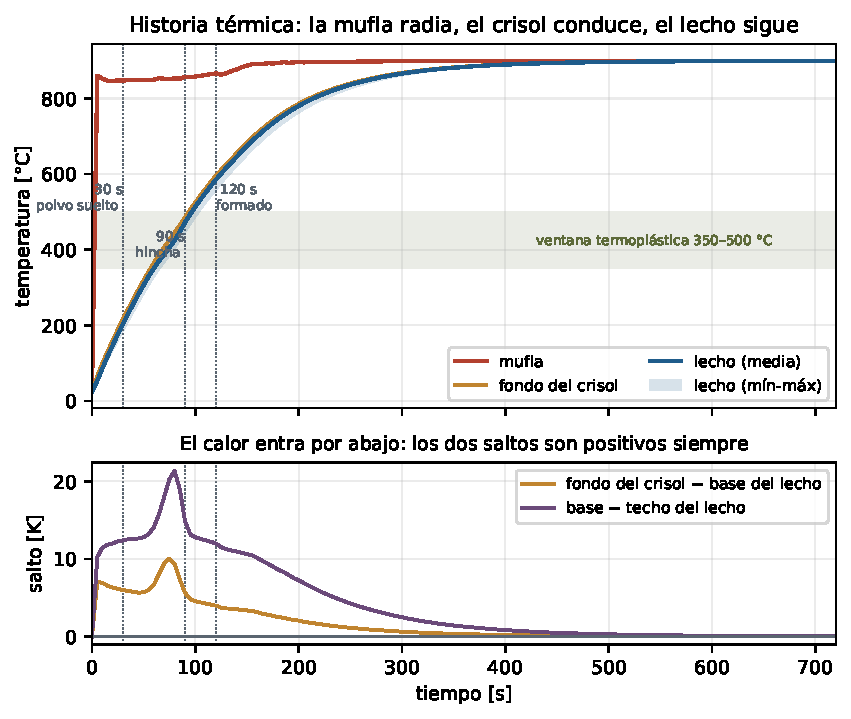
\includegraphics[width=0.82\linewidth]{fig_fen_termico.pdf}
\caption{Historia térmica. Arriba, las temperaturas; la banda gris es la
ventana termoplástica del carbón. Abajo, los dos saltos térmicos que empujan el
calor hacia dentro: ambos son positivos en todo instante, de modo que el calor
entra siempre por el fondo y sube. El pico hacia \SI{85}{\second} es la
pirólisis, que es endotérmica y frena el calentamiento del lecho justo cuando
más gas está soltando.}
\label{fig:termico}
\end{figure}

\begin{clave}
\textbf{El lecho se calienta desde abajo.} El fondo del crisol es la vía
principal: está en contacto directo con la base del lecho y es la parte más
maciza. El perfil vertical decrece de forma monótona desde el fondo hacia
arriba en todo instante. La pared lateral sólo toca el lecho en sus
\SI{3}{\milli\meter} de altura; por encima de esa cota lo que hay al otro lado
es gas, que conduce mal.
\end{clave}

\subsection{Los tiempos}

Tres escalas distintas gobiernan el arranque:

\begin{itemize}[nosep,leftmargin=*]
  \item \textbf{0--\SI{30}{\second}}: el crisol se calienta, el lecho apenas.
        A los \SI{30}{\second} el lecho está a
        \datTLechoTreinta{} \si{\celsius}: todavía no ha pasado nada
        químicamente. Coincide
        con la observación de laboratorio de que a los \SI{30}{\second} el
        material sigue siendo polvo suelto.
  \item \textbf{\SI{60}{}--\SI{120}{\second}}: el lecho cruza la ventana
        termoplástica (350--\SI{500}{\celsius}) y la compuerta de
        devolatilización (\SI{450}{\celsius}). Aquí ocurre \emph{todo}.
  \item \textbf{$>$\SI{150}{\second}}: el lecho se acerca asintóticamente a la
        mufla. A \SI{720}{\second} la diferencia entre el fondo del crisol y el
        techo del lecho es de décimas de kelvin: el sistema es isotermo.
\end{itemize}

\begin{figure}[H]\centering
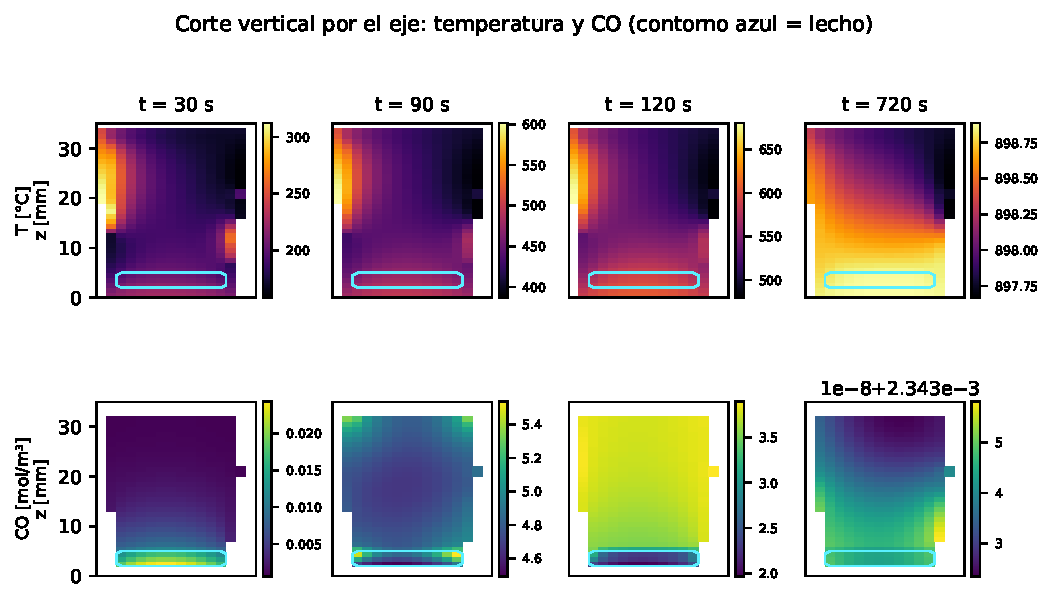
\includegraphics[width=\linewidth]{fig_fen_campos.pdf}
\caption{Corte vertical por el eje. Arriba la temperatura, abajo el CO; el
contorno azul marca el lecho. Se ve la pastilla en el fondo y el frente térmico
entrando por el cuerpo del crisol. A \SI{720}{\second} la escala de temperatura
abarca poco más de un kelvin en todo el dominio.}
\label{fig:campos}
\end{figure}

% =====================================================================
\section{Momentum, calor y masa: quién manda}

Las tres transferencias están acopladas, pero no pesan lo mismo. La forma
limpia de decidirlo es con los números adimensionales, que el solucionador
calcula celda a celda con las propiedades reales de cada instante.

\begin{table}[H]\centering\small
\caption{Números adimensionales al final de la corrida, y lo que implica cada
uno. Todos comparan un mecanismo con otro: por debajo de 1 gana el denominador.
Se dan el máximo de toda la corrida y el valor final, porque no coinciden: el
estallido de devolatilización levanta los Péclet por encima de 1 durante unos
treinta segundos.}
\begin{tabular}{llrrll}
    \hline
    Número & Símb. & Máximo & A 720 s & Compara & Consecuencia \\
    \hline
    Re de partícula & Re$_p$ & 0,39 & $5,92\times10^{-9}$ & inercia / viscosidad en el poro & flujo de Darcy, sin inercia \\
    Péclet térmico & Pe$_T$ & 3,93 & $5,90\times10^{-8}$ & advección / conducción & el calor se conduce \\
    Péclet másico & Pe$_m$ & 5,88 & $8,82\times10^{-8}$ & advección / difusión & las especies difunden \\
    Damköhler & Da & $1,60\times10^{-17}$ & $1,60\times10^{-17}$ & reacción / transporte & no hay control por transporte \\
    Rayleigh & Ra & 1861,80 & 1861,80 & boyancia / difusión & roza el umbral 1708 \\
    \hline
\end{tabular}

\end{table}

\begin{figure}[H]\centering
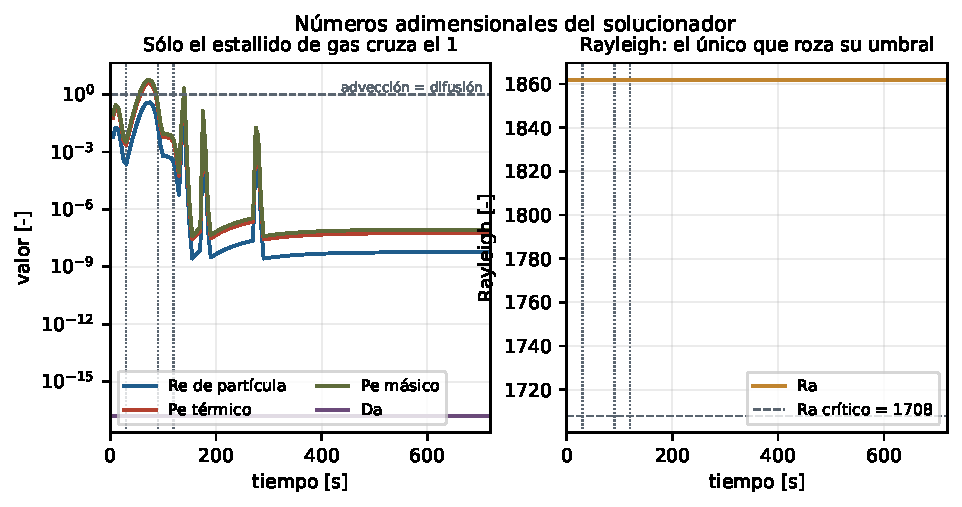
\includegraphics[width=\linewidth]{fig_fen_adimensionales.pdf}
\caption{Evolución de los adimensionales. El pico hacia \datTPico{} \si{\second}
es la devolatilización: mientras el carbón suelta gas hay velocidad, y los
Péclet suben más de cinco órdenes de magnitud y \emph{cruzan} el 1. Fuera de
esa ventana de unos treinta segundos vuelven a ser despreciables.}
\label{fig:adim}
\end{figure}

\subsection{Momentum}

La velocidad máxima del gas al final es \datUmax{}
\si{\meter\per\second}: décimas de micra por segundo. El Reynolds de partícula
queda en $10^{-6}$, así que el flujo es puramente viscoso (Darcy) y el término
inercial de Forchheimer no interviene.

\textbf{En qué afecta:} casi nada durante casi toda la corrida, y mucho durante
un rato corto. El episodio en que el momentum importa es la devolatilización:
hacia \datTPico{} \si{\second} el carbón genera gas dentro del poro, eso levanta
una sobrepresión local y empuja el gas hacia la junta de la tapa, por donde
ventea. Ahí el Reynolds de partícula llega a \datRepMax{} ---todavía viscoso,
pero cinco órdenes por encima de su valor final--- y ese venteo es el que se
lleva la masa perdida.

\subsection{Calor}

Al final $\mathrm{Pe}_T \sim 10^{-5}$: la advección de calor por el gas es cinco
órdenes de magnitud menor que la conducción. Pero en el pico de la
devolatilización $\mathrm{Pe}_T$ alcanza \datPeTermicoMax{}: durante esos
segundos el gas que sale \emph{sí} arrastra calor más rápido de lo que el lecho
lo conduce.

\textbf{En qué afecta:} fuera de esa ventana, el calor se transmite por
conducción y punto, y la temperatura del lecho es la que le impone el crisol a
través del contacto. Dentro de ella hay que contar además con el gas: es una de
las razones de que el lecho se frene hacia los \SI{85}{\second}, junto con el
calor endotérmico de pirólisis. No hay, en cambio, convección natural en ningún
momento.

Queda un matiz honesto. El Rayleigh que calcula el solucionador es
\datRa{}, y su valor crítico
\datRaCritico{}: está un \SI{9}{\percent} \emph{por
encima} del umbral de convección natural. El caso, sin embargo, tiene la
boyancia desactivada, y la justificación escrita en el archivo del caso dice
que el Rayleigh del ensayo está por debajo del umbral. Las dos cosas no
concuerdan (véase §\ref{sec:limites}). El efecto práctico es pequeño ---con
$\mathrm{Pe}_T \sim 10^{-5}$, aunque arrancara una celda convectiva débil la
conducción seguiría dominando por varios órdenes---, pero la justificación, tal
como está escrita, no se sostiene con el número que produce esta corrida.

\subsection{Masa}

Al final $\mathrm{Pe}_m \sim 10^{-5}$, y en el pico llega a
\datPeMasicoMax{}: es el número que más se despega, porque el gas que empuja es
precisamente el que transporta las especies. El Damköhler, en cambio, es
$\sim 10^{-17}$ de principio a fin.

\textbf{En qué afecta:} fuera del estallido las especies se mueven por difusión,
no arrastradas; durante el estallido, el gas de pirólisis las barre hacia la
salida. Y el Damköhler minúsculo dice algo importante y a menudo malentendido: la
reacción es \emph{lentísima} comparada con el transporte. No hay control por
difusión. Cuando una reacción no avanza en este sistema, no es porque al
reactivo le cueste llegar: es porque la termodinámica no la deja, o porque la
cinética es despreciable a esa temperatura. Ésta es la clave para entender la
ilmenita.

% =====================================================================
\section{Qué cambia de fase y qué no}

\begin{table}[H]\centering\small
\caption{Inventario de fases sólidas al principio y al final. La columna de
resultado sale de comparar las dos masas, no de una expectativa: «no cambia»
significa que la variación queda por debajo de una parte en cien mil, o de
\SI{0.1}{\micro\gram} en términos absolutos. Ambos umbrales están muy por
debajo de lo que vería una balanza.}
\begin{tabular}{lrrrl}
    \hline
    Fase & $m(0)$ [mg] & $m(720)$ [mg] & $\Delta m$ [mg] & Resultado \\
    \hline
    Volátil del carbón & 264,75 & 31,77 & -232,98 & se consume \\
    Carbono fijo (char) & 404,55 & 404,55 & 0,00 & no cambia \\
    Hematita Fe$_2$O$_3$ & 30,26 & 0,00 & -30,26 & se consume \\
    Magnetita Fe$_3$O$_4$ & 192,12 & 178,73 & -13,39 & se consume \\
    Wüstita FeO & 0,00 & 32,62 & 32,62 & se forma \\
    Hierro metálico Fe & 0,00 & 5,50 & 5,50 & se forma \\
    Ilmenita FeTiO$_3$ & 27,62 & 27,62 & 0,00 & no cambia \\
    Rutilo TiO$_2$ & 0,00 & 0,00 & 0,00 & no cambia \\
    Cuarzo SiO$_2$ & 0,00 & 0,00 & 0,00 & no cambia \\
    Fayalita Fe$_2$SiO$_4$ & 0,00 & 0,00 & 0,00 & no cambia \\
    Cenizas & 73,95 & 73,95 & 0,00 & no cambia \\
    \hline
\end{tabular}

\end{table}

\begin{figure}[H]\centering
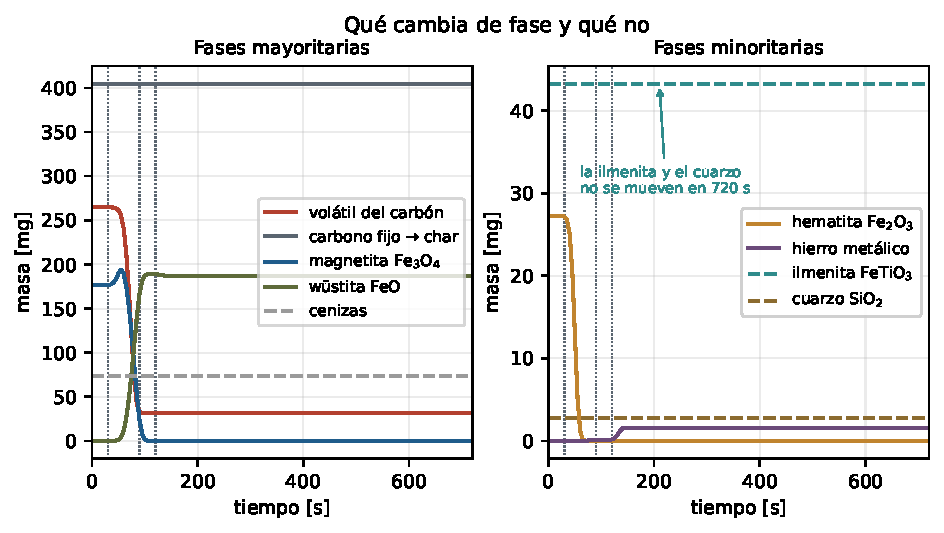
\includegraphics[width=\linewidth]{fig_fen_fases.pdf}
\caption{Evolución de las fases sólidas. Todo el movimiento ocurre entre
\SI{60}{} y \SI{130}{\second}. La ilmenita y el cuarzo son líneas rectas de
principio a fin.}
\label{fig:fases}
\end{figure}

\subsection{Lo que se transforma}

\paragraph{El volátil del carbón.} Es el gran protagonista. Cae de
\datVolatilInicial{} \si{\milli\gram} a \datVolatilFinal{} \si{\milli\gram}.
Sale como CH$_4$, H$_2$,
H$_2$O, CO y CO$_2$, y es lo que se pierde por la junta de la tapa. No es una
reacción con la magnetita: es pirólisis del carbón, que ocurriría igual sin
mineral presente.

\paragraph{La cascada del hierro.} Los óxidos se reducen en el orden que impone
la termodinámica, cada uno más difícil que el anterior:
\[
\mathrm{Fe_2O_3} \;\longrightarrow\; \mathrm{Fe_3O_4}
\;\longrightarrow\; \mathrm{FeO} \;\longrightarrow\; \mathrm{Fe}
\]
La hematita desaparece por completo (\datHematitaInicial{} \si{\milli\gram}
$\to$ 0): su frontera de reducción está tres órdenes de magnitud por debajo del
gas del lecho, así que no tiene defensa. Pero la cascada \textbf{se detiene
ahí}. La magnetita \textbf{sobrevive al ensayo}: pasa de
\datMagnetitaInicial{} a \datMagnetitaFinal{} \si{\milli\gram}, un
\datMagnetitaVariacion{}\,\%. Son dos efectos que se restan --- gana el hierro
que suelta la hematita y pierde una parte al pasar a wüstita ---, y el saldo es
una merma pequeña. La wüstita se queda en \datFeo{} \si{\milli\gram} y el hierro
metálico en \datFe{} \si{\milli\gram}, el \datPctFeMetal{}\,\% del hierro en
masa.

La razón es que el gas se tampona \emph{sobre} la frontera Fe$_3$O$_4$/FeO: al
reducir la hematita se oxida, la afinidad cae a cero y la reducción se para
donde coexisten las dos fases. Esa frontera está en CO/(CO+CO$_2$) =
\datUmbralMagnetita{}\,\% a \SI{900}{\celsius}, y el gas del lecho acaba en
\datGas{}\,\%. Es un resultado, no un ajuste: sale con los parámetros por
omisión.

\ojo{Aquí había un defecto grave, y lo destapó la prueba del imán.} La versión
anterior de este documento decía que la magnetita desaparecía por completo,
porque la termodinámica ponía esa frontera en \qty{0.76}{\percent} de CO en vez
de \qty{32}{\percent}: un factor 42, resultado de extrapolar el $C_p$ de la
magnetita fuera de su rango y de usar FeO estequiométrico en lugar de wüstita
Fe$_{0{,}947}$O. Con la frontera baja, cualquier gas reducía toda la magnetita
y el aglomerado salía no magnético, que es justo lo contrario de lo observado.

\begin{figure}[H]\centering
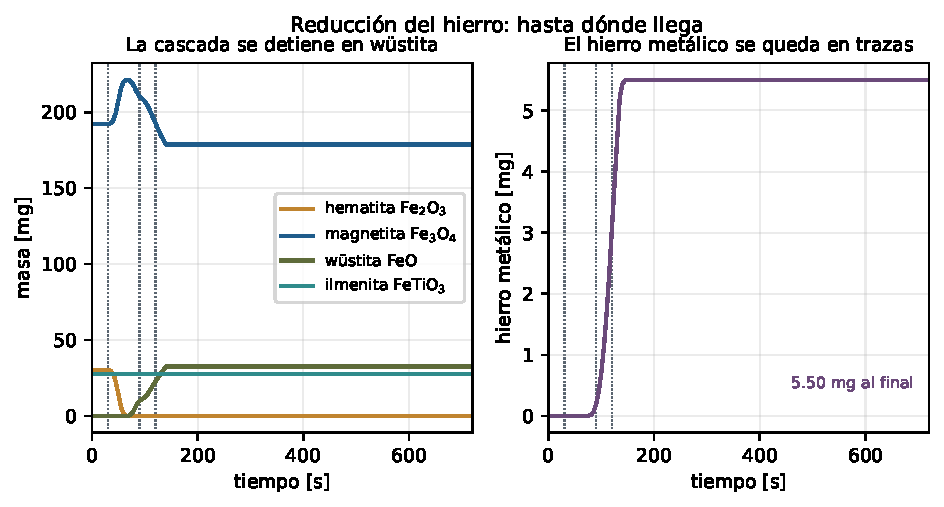
\includegraphics[width=\linewidth]{fig_fen_hierro.pdf}
\caption{La cascada se detiene en la magnetita, que sobrevive al ensayo. A la
derecha, el hierro metálico en su propia escala: son trazas.}
\label{fig:hierro}
\end{figure}

\subsection{Lo que no se mueve: la ilmenita}

\begin{clave}
La ilmenita empieza en \datIlmenita{} \si{\milli\gram} y termina en
\datIlmenita{} \si{\milli\gram}. No cambia: la diferencia que devuelve la
corrida es \emph{exactamente} cero, no una cantidad pequeña.
\end{clave}

\noindent
La razón no es cinética ni de transporte ---ya vimos que el Damköhler descarta
el control por difusión---: es \textbf{termodinámica}, y se puede poner un
número encima.

Toda reducción por CO tiene la forma general
\[
\mathrm{MO_{(s)}} + \mathrm{CO_{(g)}} \;\rightleftharpoons\;
\mathrm{M_{(s)}} + \mathrm{CO_{2(g)}},
\qquad
K = \frac{p_{\mathrm{CO_2}}}{p_{\mathrm{CO}}} .
\]
El equilibrio se alcanza cuando la fracción $x_{\mathrm{CO}} =
\mathrm{CO}/(\mathrm{CO}+\mathrm{CO_2})$ vale $1/(1+K)$. Por encima de ese
valor el gas es lo bastante reductor y la reacción avanza; por debajo, no
avanza \emph{aunque haya carbono de sobra y todo el tiempo del mundo}. Cada
óxido tiene su umbral, y son muy distintos entre sí (tabla~\ref{tab:fronteras}).

\begin{table}[H]\centering\small
\caption{Fracción mínima de CO que exige cada reducción a \SI{900}{\celsius},
calculada con las tablas termodinámicas del propio simulador. La última columna
compara con el gas que realmente hay en la corrida
(\datGas{}\,\%).}
\label{tab:fronteras}
\begin{tabular}{lrc}
    \hline
    Reducción & CO/(CO+CO$_2$) mínimo [\%] & ¿Ocurre? \\
    \hline
    Fe$_2$O$_3 \rightarrow$ Fe$_3$O$_4$ & 0,00 & sí \\
    Fe$_3$O$_4 \rightarrow$ FeO & 32,22 & \textbf{no} \\
    FeO $\rightarrow$ Fe & 70,91 & \textbf{no} \\
    FeTiO$_3 \rightarrow$ Fe + TiO$_2$ & 94,66 & \textbf{no} \\
    \hline
\end{tabular}

\end{table}

\begin{figure}[H]\centering
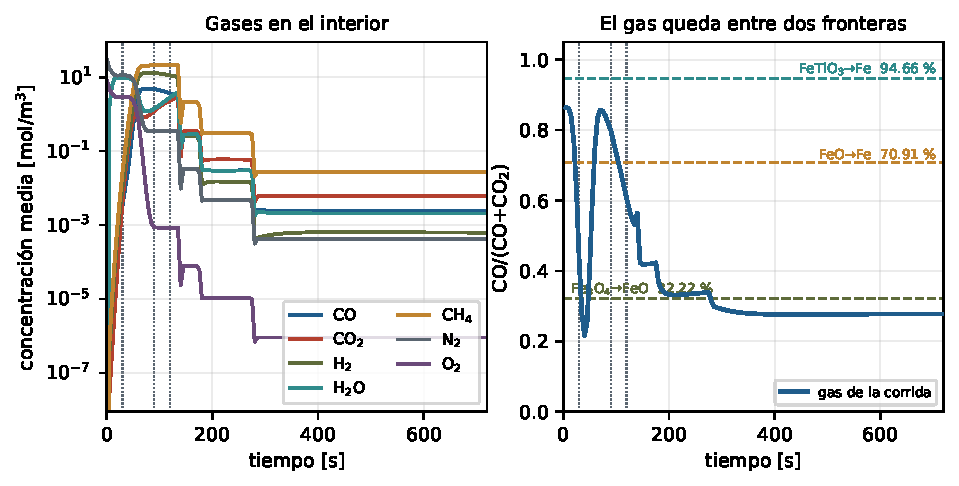
\includegraphics[width=\linewidth]{fig_fen_gases.pdf}
\caption{Izquierda: los gases del interior. Derecha: la razón
CO/(CO+CO$_2$) frente a las tres fronteras. El gas se \emph{clava} sobre la de
la magnetita ---no la cruza, se apoya en ella--- y se queda muy lejos de la de
la ilmenita. Ése es todo el argumento.}
\label{fig:gases}
\end{figure}

\noindent
La ilmenita exige \datUmbralIlmenita{}\,\% de CO. El gas
ofrece \datGas{}\,\%. La diferencia es de decenas de puntos porcentuales, y no
es algo que se cierre esperando más tiempo: es el estado de equilibrio del
sistema. Para reducir la ilmenita habría que subir la temperatura bastante por
encima de \SI{900}{\celsius}, o cambiar la atmósfera.

Hay además una razón estructural que agrava lo anterior y que viene del DRX.
En este concentrado el titanio no está como ilmenita libre sino dentro de una
\emph{titanohematita}, un miembro intermedio de la serie hematita--ilmenita
($x = 0{,}49$), y esa fase está \emph{intercrecida dentro de los granos de
magnetita}. El propio refinamiento lo respalda: su tamaño aparente de
cristalito es \SI{22.8}{\nano\meter} en la fracción magnética frente a
\SI{83.3}{\nano\meter} en la no magnética, que es la firma de unas lamas finas
de exsolución frente a granos sueltos. Aunque la termodinámica lo permitiera,
ese hierro está peor expuesto que el de la magnetita que lo hospeda.

\paragraph{Cuarzo y cenizas.} No cambian por la misma clase de razón: no hay
ninguna ruta accesible a \SI{900}{\celsius}. Y la fayalita
(Fe$_2$SiO$_4$), que a veces se invoca para explicar la cohesión, se mantiene
en cero: funde a \SI{1178}{\celsius}, casi trescientos grados por encima del
ensayo. \textbf{No hay escoria líquida en este ensayo.}

\subsection{Qué se recupera: las fases a temperatura ambiente}
\label{sec:enfriado}

Todo lo anterior es el estado \emph{dentro} de la mufla. Lo que el laboratorio
tiene en la mano es otra cosa, porque entre los \SI{900}{\celsius} y la mesa hay
una transformación que sí ocurre: por debajo de \SI{570}{\celsius} la wüstita
deja de ser estable y se descompone,
$4\,\mathrm{FeO} \rightarrow \mathrm{Fe_3O_4} + \mathrm{Fe}$.

Es la \emph{única} que hay. La ilmenita, la titanohematita, el char y las
cenizas no tienen ninguna ruta accesible en ese intervalo, así que bajan
congelados.

\begin{table}[H]
\centering\small
\begin{tabular}{rrrrrrrrrrr}
    \hline
     &  &  & \multicolumn{8}{c}{\% en masa del sólido} \\
    $t$ [s] & masa [mg] & $\varepsilon$ & volátil & char & ceniza & Fe$_2$O$_3$ & Fe$_3$O$_4$ & FeO & Fe & FeTiO$_3$ \\
    \hline
    0 & 993,2 & 0,540 & 26,65 & 40,73 & 7,45 & 3,05 & 19,34 & 0,00 & 0,00 & 2,78 \\
    30 & 993,2 & 0,540 & 26,65 & 40,73 & 7,45 & 3,04 & 19,35 & 0,00 & 0,00 & 2,78 \\
    60 & 968,6 & 0,552 & 24,89 & 41,77 & 7,63 & 0,13 & 22,73 & 0,00 & 0,00 & 2,85 \\
    90 & 759,5 & 0,677 & 4,33 & 53,26 & 9,74 & 0,00 & 27,70 & 1,31 & 0,02 & 3,64 \\
    120 & 756,4 & 0,678 & 4,20 & 53,48 & 9,78 & 0,00 & 25,50 & 2,99 & 0,41 & 3,65 \\
    150 & 754,7 & 0,678 & 4,21 & 53,60 & 9,80 & 0,00 & 23,68 & 4,32 & 0,73 & 3,66 \\
    210 & 754,7 & 0,678 & 4,21 & 53,60 & 9,80 & 0,00 & 23,68 & 4,32 & 0,73 & 3,66 \\
    360 & 754,7 & 0,678 & 4,21 & 53,60 & 9,80 & 0,00 & 23,68 & 4,32 & 0,73 & 3,66 \\
    720 & 754,7 & 0,678 & 4,21 & 53,60 & 9,80 & 0,00 & 23,68 & 4,32 & 0,73 & 3,66 \\
    \hline
\end{tabular}

\caption{Inventario de fases \textbf{dentro de la mufla}, en \si{\milli\gram},
para cada instante de extracción. A partir de los \SI{150}{\second} no cambia
nada más: se agotó el reductor.}
\label{tab:fases-tiempo}
\end{table}

\begin{table}[H]
\centering\small
\begin{tabular}{rrrrrrrrr}
    \hline
     & \multicolumn{2}{c}{Fe$_3$O$_4$ [mg]} & \multicolumn{2}{c}{FeO [mg]} & \multicolumn{2}{c}{Fe [mg]} & \multicolumn{2}{c}{$M_s$ [A m$^2$/kg]} \\
    $t$ [s] & temple & lento & temple & lento & temple & lento & temple & lento \\
    \hline
    0 & 192,1 & 192,1 & 0,0 & 0,0 & 0,00 & 0,00 & 17,8 & 17,8 \\
    30 & 192,2 & 192,2 & 0,0 & 0,0 & 0,00 & 0,00 & 17,9 & 17,9 \\
    60 & 220,1 & 220,1 & 0,0 & 0,0 & 0,00 & 0,00 & 21,0 & 21,0 \\
    90 & 210,4 & 218,4 & 10,0 & 0,0 & 0,19 & 2,13 & 25,7 & 27,2 \\
    120 & 192,9 & 211,1 & 22,6 & 0,0 & 3,07 & 7,46 & 24,5 & 27,9 \\
    150 & 178,7 & 205,0 & 32,6 & 0,0 & 5,50 & 11,83 & 23,5 & 28,5 \\
    210 & 178,7 & 205,0 & 32,6 & 0,0 & 5,50 & 11,84 & 23,5 & 28,5 \\
    360 & 178,7 & 205,0 & 32,6 & 0,0 & 5,50 & 11,84 & 23,5 & 28,5 \\
    720 & 178,7 & 205,0 & 32,6 & 0,0 & 5,50 & 11,84 & 23,5 & 28,5 \\
    \hline
\end{tabular}

\caption{Lo que se \textbf{recupera a temperatura ambiente}, según qué le pase a
la wüstita al enfriar. «Temple» la conserva entera; «lento» la descompone del
todo en magnetita y hierro. La lectura real está entre las dos columnas, y más
cerca de la de temple cuanto más rápido se enfríe. Las fases que no aparecen
---volátil, char, ceniza, ilmenita--- son las mismas del
cuadro~\ref{tab:fases-tiempo}: no cambian al enfriar.}
\label{tab:enfriado}
\end{table}

\paragraph{Dónde cae este ensayo entre las dos columnas.} Con la curva de
enfriamiento del crisol, el cuerpo pasa \datEnfriaVentana\ \si{\second} dentro
de la ventana en que el eutectoide puede operar. Aplicando una ley de
Avrami anclada en las dos únicas fracciones medidas que se han encontrado
(Zorc, Nagode y Kosec, 2024: \num{0.17} de wüstita retenida enfriando a
\SI{100}{\celsius\per\minute} y \num{0.41} a \SI{1000}{\celsius\per\minute}),
sale que se descompondría en torno al \datFraccionEutectoide\,\% de la wüstita:
más o menos a mitad de camino entre las dos columnas.

\ojo{Ese número no es un resultado, es una ilustración.} Depende de un supuesto
sobre cuánta wüstita había en las probetas de esa referencia, y sus muestras son
capas de óxido sobre acero, no un aglomerado carbón--mineral. El resultado que
este informe defiende son \textbf{las dos cotas}; el valor intermedio sólo dice
que el caso real no está pegado a ninguna de ellas.

\paragraph{Lo que el enfriado hace y este modelo no recoge.} Tres cosas, y las
tres se declaran porque van en direcciones distintas:

\begin{itemize}[leftmargin=*,itemsep=2pt]
\item \textbf{Reoxidación en aire.} El aglomerado sale a \SI{900}{\celsius} y se
enfría al aire. Su superficie puede reoxidarse ---magnetita a hematita o
maghemita, hierro metálico a óxido---, lo que restaría magnetismo a las dos
cotas, y más a la de enfriamiento lento, que pasa más tiempo caliente.
\item \textbf{Combustión del char.} Quedan \datCarbono\ \si{\milli\gram} de
carbono fijo y salen al aire incandescentes. Lo que arda quita masa \emph{no}
magnética y por tanto \emph{sube} la magnetización específica sin cambiar
ninguna fase de hierro.
\item \textbf{Gradientes dentro del cuerpo.} La curva de enfriamiento es de
capacidad concentrada: da una sola temperatura. La superficie cruza el
eutectoide antes que el núcleo, así que la descomposición no es uniforme y el
DRX de un polvo molido daría una media de estados distintos.
\end{itemize}

\noindent
Las tres se cierran con la misma medida: un DRX del aglomerado recuperado, a dos
o tres tiempos. Es lo que convertiría el cuadro~\ref{tab:enfriado} de predicción
en resultado.

% =====================================================================
\section{Por qué se congelan las composiciones}

Mirando la figura~\ref{fig:fases}, todo el movimiento químico ocurre en una
ventana de unos \SI{70}{\second} y después las líneas son rectas. Hay tres
razones superpuestas, y conviene no confundirlas:

\begin{enumerate}[leftmargin=*]
  \item \textbf{Se acaba el reactivo que se estaba consumiendo.} La hematita y
        la magnetita se agotan literalmente: llegan a cero. Una reacción sin
        reactivo se para sola.
  \item \textbf{Se llega a una frontera termodinámica.} La wüstita sí queda
        ---\datFeo{} \si{\milli\gram}--- y hay carbono de
        sobra (\datCarbono{} \si{\milli\gram}, intacto), pero el gas no es lo bastante
        reductor para pasar de ahí. Esto no es agotamiento: es un tope.
  \item \textbf{Se acaba el volátil.} La devolatilización es la que genera el
        gas; cuando el volátil liberable se agota, la fuente se apaga y el
        sistema queda en el estado en que estaba.
\end{enumerate}

\noindent
El punto 2 es el importante y el que más se malinterpreta. \textbf{Que sobre
carbono no significa que la reducción pueda continuar.} El carbono fijo termina
en \datCarbono{} \si{\milli\gram}, que es lo mismo con que empezó salvo una
parte en diez millones. No se consume porque la reacción de Boudouard
(C + CO$_2$ $\rightarrow$ 2\,CO), que es la que
regeneraría el CO, es demasiado lenta \emph{en el modelo} a esta temperatura
para mover el sistema en \SI{720}{\second}.

\ojo{Y ahí está la discrepancia abierta del trabajo.} El laboratorio observa que
el aglomerado sigue perdiendo respuesta al imán cuanto más tiempo pasa en la
mufla, y este modelo no lo reproduce: congelado a los \SI{150}{\second}, predice
que un aglomerado de \SI{300}{\second} y otro de \SI{720}{\second} responden
igual. Para que siguiera reduciéndose haría falta CO, y el único carbono
disponible es precisamente este char. La constante \texttt{k\_boudouard} es uno
de los parámetros que la calibración declara \textbf{no identificables} con la
curva de pérdida de masa; la prueba del imán sí podría identificarla. No se ha
tocado: queda registrada como discrepancia, no ajustada.

% =====================================================================
\section{Por qué deja de perder masa}

\begin{figure}[H]\centering
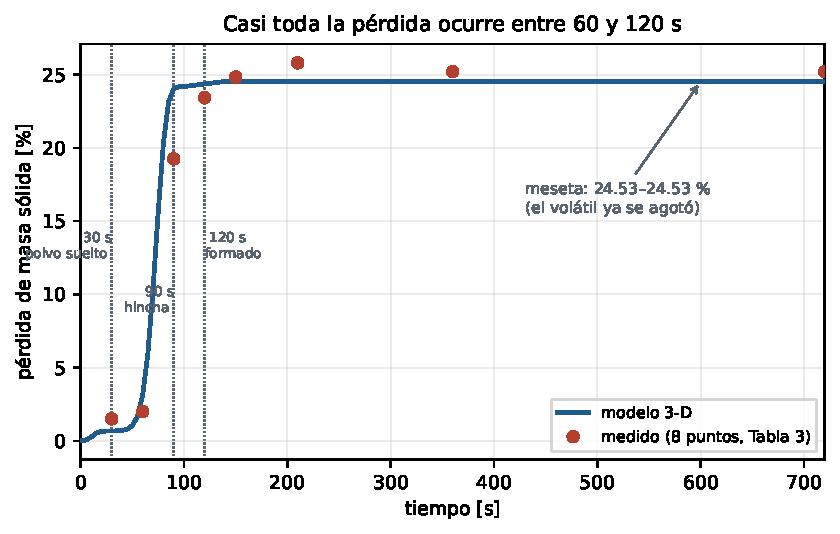
\includegraphics[width=0.82\linewidth]{fig_fen_perdida.pdf}
\caption{Pérdida de masa. La curva del modelo cae sobre los ocho puntos
medidos sin haber sido ajustada a ellos.}
\label{fig:perdida}
\end{figure}

\noindent
La pérdida final es \datPerdidaFinal{}\,\%, frente al
\SI{25.20}{\percent} medido a \SI{720}{\second}. Y alcanza el
\SI{99}{\percent} de su valor final a los
\datTMeseta{} \si{\second}: a partir de ahí la curva es
plana (\datMeseta{}\,\% entre \SI{300}{} y
\SI{720}{\second}).

\begin{clave}
\textbf{La pérdida de masa no mide la reducción.} Prácticamente toda es
devolatilización del carbón. El oxígeno arrancado a los óxidos es una fracción
mínima del total, y va sumado a lo mismo que se mide en la balanza.
\end{clave}

\noindent
La consecuencia metodológica es seria y conviene decirla sin rodeos: se puede
ajustar muy bien la curva de pérdida de masa ---un $R^2$ alto--- y no haber
demostrado nada sobre las fases. Un ajuste de Gompertz sobre estos ocho puntos
caracteriza la \emph{pirólisis}, no la reducción. De hecho, con estos ocho datos
el grado de reducción no es identificable: puede variar en un rango amplio sin
que el ajuste empeore de forma apreciable.

Por eso el argumento de este documento sobre las fases \textbf{no se apoya en la
curva de pérdida de masa} sino en la termodinámica de la
tabla~\ref{tab:fronteras}, que es independiente de ella.

Y ahí está la razón de que la curva se aplane: no queda volátil que soltar. El
sistema no ha llegado a ningún equilibrio global ---queda wüstita y queda
carbono--- simplemente se ha quedado sin la única fuente que movía la balanza.

% =====================================================================
\section{El aglomerado: cómo se forma y qué tamaño tiene}

\subsection{De polvo a cuerpo}

La cohesión de este sistema \textbf{es coquización del carbón}, no puentes
metálicos ni escoria. El carbón tiene índice de hinchamiento 8 (ASTM D720): es
fuertemente coquizable. Al cruzar la ventana termoplástica (350--\SI{500}{
\celsius}) la masa se reblandece, las partículas se sueldan entre sí y al
resolidificar queda un cuerpo único con los granos minerales embebidos.

\begin{figure}[H]\centering
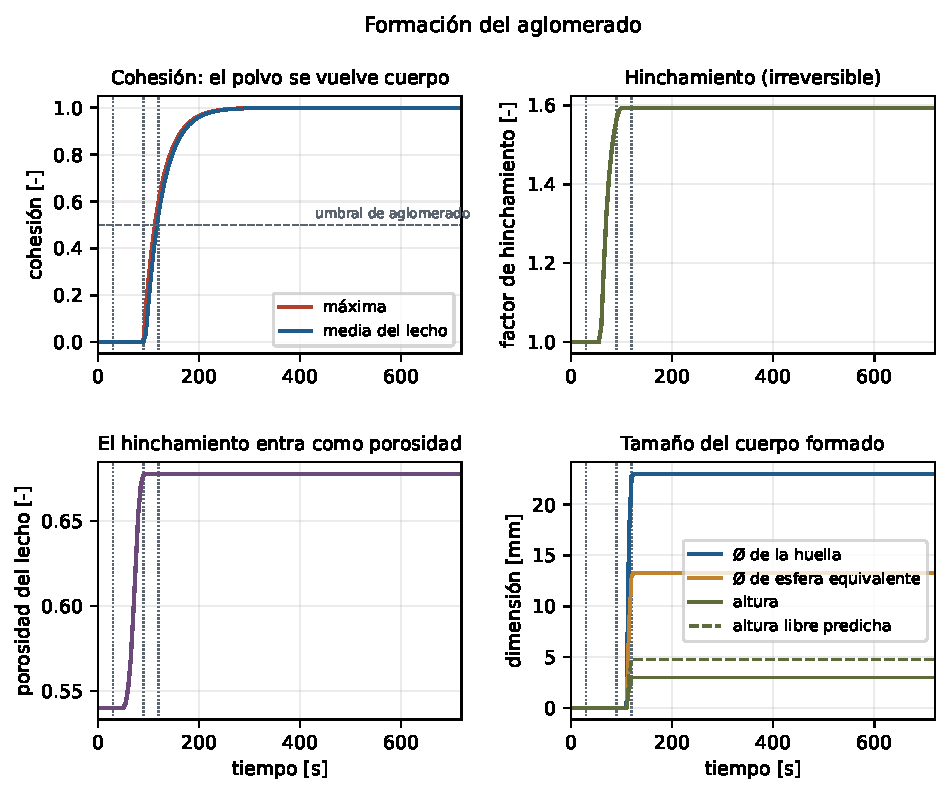
\includegraphics[width=\linewidth]{fig_fen_aglomerado.pdf}
\caption{Formación del aglomerado. La cohesión cruza el umbral operativo hacia
\datTFormacion{} \si{\second}. El hinchamiento es
irreversible: sube durante la etapa plástica y se queda.}
\label{fig:aglomerado}
\end{figure}

\begin{table}[H]\centering\small
\caption{Cronología. Cada columna sale de la corrida.}
\begin{tabular}{rrrrrrr}
    \hline
    $t$ [s] & $T_\text{lecho}$ [$^\circ$C] & pérdida [\%] & cohesión & hinch. & $\varepsilon$ & $\varnothing$ [mm] \\
    \hline
    0 & 25 & 0,00 & 0,000 & 1,000 & 0,540 & 0,0 \\
    30 & 205 & 0,68 & 0,000 & 1,000 & 0,540 & 0,0 \\
    60 & 352 & 3,21 & 0,000 & 1,039 & 0,552 & 0,0 \\
    90 & 472 & 25,19 & 0,000 & 1,563 & 0,681 & 0,0 \\
    120 & 587 & 25,47 & 0,602 & 1,594 & 0,682 & 22,8 \\
    150 & 675 & 25,51 & 0,840 & 1,594 & 0,682 & 23,0 \\
    300 & 866 & 25,51 & 0,998 & 1,594 & 0,682 & 23,0 \\
    720 & 899 & 25,51 & 1,000 & 1,594 & 0,682 & 23,0 \\
    \hline
\end{tabular}

\end{table}

\noindent
Merece la pena subrayar lo siguiente, porque es la única validación de
cronología que existe. El laboratorio aportó tres observaciones cualitativas, y
el modelo, \textbf{sin haber sido ajustado a ellas}, produce:

\begin{itemize}[nosep,leftmargin=*]
  \item a los \SI{30}{\second}, \datPerdidaTreinta{}\,\% de pérdida
        y cohesión nula
        \;---\; \emph{«polvo suelto»};
  \item a los \SI{90}{\second}, el hinchamiento ya en \datHinchamientoNoventa{}
        y la pérdida
        disparada \;---\; \emph{«se hincha»};
  \item a los \SI{120}{\second}, cohesión por encima del umbral
        \;---\; \emph{«bien formado»}.
\end{itemize}

\subsection{El diámetro}

Ésta es la pregunta que más cuesta responder bien, porque la respuesta
más natural es la equivocada. \textbf{El aglomerado no es una esfera.} Está
confinado por la pared del crisol: no puede crecer a lo ancho, así que su
diámetro no lo fija la física del hinchamiento sino la geometría del recipiente.

\begin{table}[H]\centering\small
\caption{Dimensiones del cuerpo formado, al final de la corrida.}
\begin{tabular}{lrl}
    \hline
    Magnitud & Valor & Unidad \\
    \hline
    Instante en que se forma (cohesión $\geq$ 0,5) & 115 & s \\
    Diámetro de la huella & 23,0 & mm \\
    Altura resuelta & 3,0 & mm \\
    Altura libre predicha (hinchado) & 4,8 & mm \\
    Volumen aparente & 1232 & mm$^3$ \\
    Volumen de materia sólida & 402 & mm$^3$ \\
    Diámetro de esfera de igual volumen & 13,3 & mm \\
    Porosidad final & 0,678 & --- \\
    Factor de hinchamiento & 1,594 & --- \\
    Diámetro de partícula de partida & 0,175 & mm \\
    \hline
\end{tabular}

\end{table}

\begin{clave}
\textbf{Respuesta.} El aglomerado formado es un disco de
\textbf{\datDiametro{} \si{\milli\meter} de diámetro} y
\textbf{\datAltura{} \si{\milli\meter} de altura}. El diámetro lo impone la
pared del crisol: el cuerpo empieza a cuajar hacia \datTFormacion{}
\si{\second}, alcanza el ancho del crisol en los diez segundos siguientes, y a
partir de ahí \emph{no vuelve a cambiar} hasta los \SI{720}{\second}.
\end{clave}

\noindent
Si lo que se busca es un número comparable con el tamaño de partida, hay dos
formas legítimas de darlo, y conviene no mezclarlas:

\begin{itemize}[leftmargin=*]
  \item \textbf{Diámetro de esfera equivalente}: la esfera que tendría el mismo
        volumen aparente es de \datDesfe{}
        \si{\milli\meter}. Sirve para comparar con las partículas de partida,
        de \SI{175}{\micro\meter}: el cuerpo formado es unas
        \textbf{\datCrecimientoLineal{} veces mayor en escala lineal}, y unas
        \datCrecimientoVolumen{} veces en volumen. Ése es el salto que significa
        «aglomerar».
  \item \textbf{Altura, que es lo que sí crece}: como la pared impide la
        expansión radial, todo el hinchamiento se resuelve hacia arriba. Con un
        factor de hinchamiento de \datHinchamiento{}, la superficie libre
        subiría de \datAltura{} a \datAlturaLibre{} \si{\milli\meter}.
\end{itemize}

\noindent
Hay que ser explícito sobre un límite del modelo aquí. La malla del simulador es
\textbf{fija}: el lecho ocupa siempre las mismas celdas. El hinchamiento no
entra haciendo crecer el cuerpo hacia arriba, sino \textbf{aumentando la
porosidad} de esas celdas, que pasa de \datEpsInicial{} a
\datEpsFinal{}. Es consistente ---el volumen de materia sólida por
el complemento de la porosidad reproduce el inventario de fases--- pero
significa que la altura de \datAlturaLibre{}
\si{\milli\meter} es una \emph{predicción del submodelo de hinchamiento}, no
algo que el 3-D resuelva moviendo la superficie.

% =====================================================================
\section{Límites de lo que aquí se afirma}
\label{sec:limites}

Este documento sería deshonesto sin esta sección.

\paragraph{Ninguna fase está validada \emph{directamente}.} Toda la
caracterización instrumental del material (DRX-Rietveld) es \emph{previa} al
ensayo. La predicción de que el producto es magnetita con algo de wüstita y la
ilmenita intacta se apoya en una sola observación, y cualitativa: que el
aglomerado sigue pegándose al imán. Basta con eso para descartar que la
magnetita se agote ---y así se descartó---, pero no para fijar el reparto entre
las fases. Un DRX o un Mössbauer del aglomerado \emph{después} del ensayo, a dos
o tres tiempos, confirmaría o tumbaría el cuadro~\ref{tab:enfriado}; es, con
diferencia, el dato que más falta hace.

\paragraph{El Rayleigh contradice su propia justificación.} El caso desactiva la
boyancia con el argumento de que el Rayleigh está por debajo del umbral
convectivo, pero el que calcula el solucionador es
\datRa{} frente a un crítico de
\datRaCritico{}: un \SI{9}{\percent} por encima. La
conclusión de que domina la conducción se sostiene igualmente por el Péclet,
pero la justificación escrita no.

\paragraph{El gas no cumple su ecuación de estado.} En el instante inicial la
suma de las concentraciones de las siete especies coincide exactamente con
$P/RT$. Al final de la corrida la supera en un factor de aproximadamente 3,4:
el modelo inyecta los productos de pirólisis sin que la densidad del gas
responda. Esto \emph{no} afecta al argumento de las fases, que descansa en la
\emph{razón} CO/(CO+CO$_2$) y no en concentraciones absolutas ---una
sobredensidad uniforme se cancela al dividir---, pero sí quiere decir que las
concentraciones absolutas de la figura~\ref{fig:gases} no deben leerse como
densidades reales.

\paragraph{El submodelo de cohesión tiene parámetros calibrables.} Los tiempos
de plastificación y coquización (\SI{15}{\second} cada uno) y la expansión por
unidad de índice de hinchamiento no son constantes medidas de esta muestra. La
cronología que reproducen es coherente con las tres observaciones del
laboratorio, pero eso es una comprobación débil, no una calibración.

\paragraph{Qué falta del laboratorio, por orden de valor.}
\begin{enumerate}[nosep,leftmargin=*]
  \item DRX / Mössbauer / SEM del aglomerado \textbf{después} del ensayo.
  \item Análisis del gas de salida (CO/CO$_2$): validaría directamente la
        figura~\ref{fig:gases}, que es el eje de todo el argumento.
  \item TGA del carbón solo, con su historia térmica medida: separaría
        devolatilización de reducción.
  \item Dilatometría de la mezcla: fijaría el factor de hinchamiento y con él
        la altura del cuerpo.
\end{enumerate}

% =====================================================================
\section{Resumen}

\begin{enumerate}[leftmargin=*]
  \item El calor entra por \textbf{radiación} de la mufla al crisol y de ahí por
        \textbf{conducción}, principalmente por el fondo. El lecho es una
        pastilla delgada y se calienta de abajo arriba.
  \item \textbf{El transporte por advección sólo cuenta durante el estallido de
        gas}. Fuera de esa ventana de unos treinta segundos, Re y Pe rondan
        $10^{-5}$--$10^{-6}$: el calor se conduce y las especies difunden. En el
        pico, hacia \datTPico{} \si{\second}, los Péclet cruzan el 1
        ($\mathrm{Pe}_m$ llega a \datPeMasicoMax{}). El Damköhler, siempre
        $\sim10^{-17}$, descarta el control por transporte en todo momento.
  \item \textbf{Cambian de fase}: el volátil del carbón (se va), la hematita y
        la magnetita (se consumen del todo) y la wüstita (se forma).
  \item \textbf{No cambian}: la ilmenita, el cuarzo, las cenizas y el carbono
        fijo. La ilmenita porque exige un gas con
        \datUmbralIlmenita{}\,\% de CO y sólo hay
        \datGas{}\,\%.
  \item \textbf{Todo ocurre entre \SI{60}{} y \SI{130}{\second}} y luego se
        congela: se agotan los óxidos reducibles, se agota el volátil, y lo que
        queda tropieza con una frontera termodinámica.
  \item \textbf{La pérdida de masa se detiene} porque se acaba el volátil, no
        porque se acabe la reducción. Los dos procesos no se distinguen en la
        balanza.
  \item \textbf{El aglomerado} es un disco de
        \datDiametro{} $\times$
        \datAltura{} \si{\milli\meter}, con el diámetro
        impuesto por el crisol, formado hacia
        \datTFormacion{} \si{\second} y estable a partir de
        ahí. La cohesión es coquización del carbón.
\end{enumerate}

\vfill
\noindent\rule{\linewidth}{0.4pt}\\
\small
Documento generado automáticamente de la corrida del simulador 3-D. Figuras y
tablas: \texttt{informe/figuras\_fenomenologia.py} y
\texttt{informe/tablas\_fenomenologia.py}. Visor interactivo de la misma
corrida: \url{https://aleramirezpo.github.io/simulador3d-carbon-magnetita/}

\end{document}
